\documentclass[11pt]{article}
\usepackage[a4paper,margin=26mm]{geometry}
\usepackage{fontspec,unicode-math,booktabs,array,graphicx,hyperref}
\setmainfont{STIXGeneral}\setmathfont{STIX Two Math}\setmonofont{Menlo}
\hypersetup{colorlinks=true,urlcolor=blue}\setlength{\parindent}{0pt}\setlength{\parskip}{5pt}\setlength{\emergencystretch}{3em}
\title{Where the affine proof costs lie}\author{\texttt{human\_compression}}\date{Exclusive text assignment; independent cost review pending}
\begin{document}\maketitle\vspace{-1em}
The accepted comparison concerns one complete historical manuscript,
Hou--Feng--Leemans, \emph{Regular 3-polytopes of order $2^np$},
arXiv:2001.02945v2 (14 July 2024), and its complete replacement: the common
paper, the application, and six whole mathematical programs. Its 33 detailed
records describe one principal contract, including retained inputs and
qualifications. They are not 33 new theorems.

The table preserves the independently accepted measurement. The ruler is
calibrated NFC characters without whitespace; all other 29 coordinates remain
in the data. These are extracted-text costs. Formula layout, unextracted
images, expanded external proofs and unavailable historical software are
unknown. No total comparison including those unknown quantities is asserted.
\begin{center}\begin{tabular}{@{}lr@{}}\toprule
Complete document & Cost \\\midrule
Historical manuscript (17 pages) & 32,767\\
Common paper (7 pages) & 19,070\\
Application (9 pages) & 22,638\\
Six complete programs, printed appendix (8 pages) & 17,250\\\bottomrule
\end{tabular}\end{center}
The whole written comparison is $32767/41708\simeq0.786$.
Including the printed programs gives $32767/58958\simeq0.556$;
using their complete raw files instead gives $32767/58390\simeq0.561$.
The raw and printed forms are alternatives, not two charges for the same code.
The replacement is longer under these whole-topic rulers.
After the \emph{whole} common paper and all six programs have been paid,
the separate conditional comparison is $32767/22638\simeq1.447$.
It does not replace the whole-topic comparison or waive the acquisition cost.

\textbf{From passages to proof routes.}
Every character belongs to exactly one of 194 owners, including four owners
for page furniture in the untrimmed coordinate. The selected texts have 190
disjoint spans. Front matter, references, connective prose, unused common
results and excluded source assertions all retain their costs. Repeated
printed statements are paid for every occurrence.

A mathematical node can refer to several owners. Two nodes may need the same
statement or presentation, so their displayed interface costs can overlap.
For a proof route we first take the logical prerequisite closure, then the
\emph{union} of its owners, and only then sum. Adding box costs would be wrong.
There is no compression factor derived from graph size or from an individual
33-row route. The full manuscript remains the denominator boundary even
where a selected proof uses only part of it.
\newpage
\textbf{The shared arguments and local work.}
The supported-kernel theorem supplies the odd-factor construction; the
application still pays for its exact commutator periods and reverse
presentation bound. The affine presentation bridge and period-intersection
criterion are reused for both cubic types. Each application supplies its
actual translation words, invariant lattice and finite overlap calculation.
The source instead rewrites three subgroups and identifies three base
quotients for each cubic type. Both graphs retain these actual dependencies;
neither substitutes invented repetitions for the source's own reuse.

Problem 1.1, the separate small-order table and the uniqueness assertion for
the two order-384 seeds remain excluded. The final odd-label existence
question was already answered historically; its complete local model is
included with attribution and no new question credit.

The exact source presentations and common theorem statements are explicitly
shared among their branches. For example, each branch of source Lemma 4.5
includes its setup and common displayed argument. Its first branch remains
flagged as false in the bound edition. The replacement proves the sign
obstruction and corrected construction. Corollary 5.2's printed reference
is also flagged. Costs do not validate either documentary defect.

The one-edge extension has an independent proof. Its comparison with the
supported-kernel theorem is not treated as a premise. The unused deletion
corollary and the smaller-period lemma remain paid in the full common paper.
Historical citations and replacement citations are treated alike: their
printed statements are measurable, while unincorporated proofs remain null.

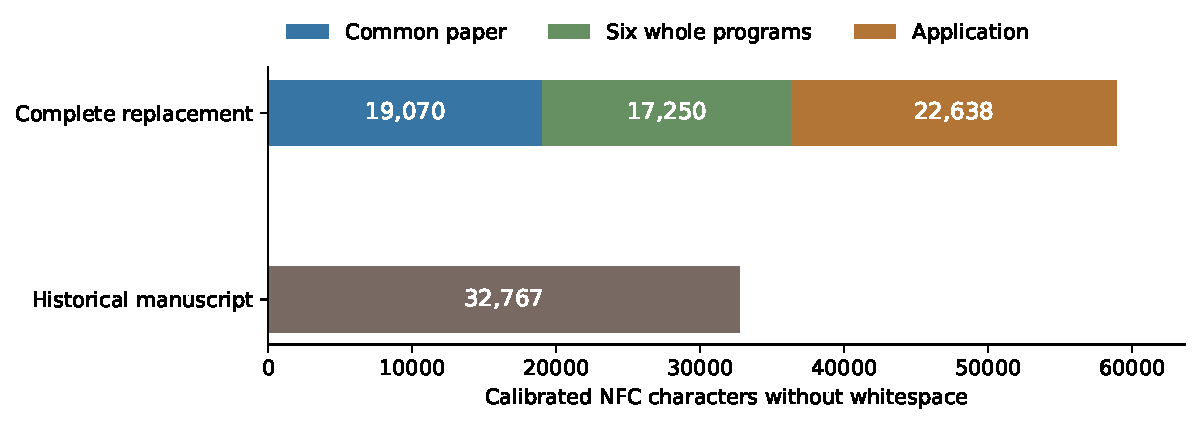
\includegraphics[width=\linewidth]{acquisition.pdf}
The drawing shows an acquisition order, not the chronology of research.
With one application, it cannot demonstrate a repeated sawtooth pattern.
Common theory reused from another topic is paid again for this independent
topic; only reuse inside this topic can use its already acquired library.

\textbf{Complete graphs and evidence.}
The linked \href{historical_graph.svg}{historical graph} and
\href{new_graph.svg}{replacement graph} show every mathematical prerequisite
edge in their respective sides, including external leaves. Arrows point from
prerequisite to use. Box labels give overlapping interface costs, not new
charges. Formal, diagnostic, operational, attribution and comparison links
are separately recorded and do not enlarge proof closures.

The six mathematical files stay whole, including embedded diagnostics.
Two drivers and one diagnostic are separately measured (16,581 raw characters);
three Lean files are also separate (7,958), with exactly nine scoped
declarations. These prove two smaller-period statements, three sign identities
and four generic quotient criteria. They do not certify affine coordinates,
actual subgroup presentations or catalogue completeness. Historical code and
algorithm/catalogue construction costs remain unknown.

\textbf{Review boundary.}
The logical graph and complete-document arithmetic have distinct prior
acceptances. The present author also reviewed that graph and authored the
canonical affine papers; this ownership assignment therefore awaits another
reviewer. Its replay verifies all 120 PDF metric cells, all whole files and
all prerequisite-owner unions. It introduces no new mathematical result,
source credit, conjecture solution or formal theorem.
\end{document}
